\subsection{Model Setup} \label{ss:model_setup}
We used the MECCA box model to determine the important gas-phase chemical processes for ozone production under different temperatures and \ce{NO_x} conditions.
The MECCA box model was set up as described in \citet{Coates:2015} and updated to include vertical mixing with the free troposphere using a diurnal cycle for the PBL height.
The supplementary material includes further details of these updates.

Simulations were performed to broadly simulate urban conditions representative of central Europe with equinoctical conditions.
The simulations started at 06:00 with a total run time of two days.
Methane was fixed at $1.7$~ppmv throughout the model run, carbon monoxide (CO) and ozone were initialised at $200$~ppbv and $40$~ppbv and then allowed to evolve freely throughout the simulation.
All VOC emissions were held constant until noon of first day simulating a plume of freshly-emitted VOC.

Separate box model simulations were performed by systematically varying the temperature between $288$ and $313$~K ($15$~--~$40$~\degree C). 
The only source of \ce{NO_x} emissions in the box model was a constant source of NO emissions. 
Box model runs were performed with the NO emissions systematically varied between $5.0~\times~10^9$ and $1.5~\times~10^{12}$~molecules~(NO)~cm$^{-2}$~s$^{-1}$ at each temperature used in this study.
At $20$~\degree C, these NO emissions corresponded to peak \ce{NO_x} mixing ratios of $0.02$~ppbv and $10$~ppbv respectively, this range of \ce{NO_x} mixing ratios covers the \ce{NO_x} conditions in pristine and urban conditions \citep{vonSchneidemesser:2015}.

All simulations were repeated using different chemical mechanisms to investigate whether the relationship of ozone with temperature across \ce{NO_x} gradients changes using different representations of ozone production chemistry.
The reference chemical mechanism was the near-explicit Master Chemical Mechanism, MCMv3.2, \citep{Jenkin:1997, Jenkin:2003, Saunders:2003, MCM_Site}.
The reduced chemical mechanisms in our study were Common Representative Intermediates, CRIv2 \citep{Jenkin:2008}, Model for ozone and related chemical tracers, MOZART-4 \citep{Emmons:2010}, Regional Acid Deposition Model, RADM2 \citep{Stockwell:1990} and the Carbon Bond Mechanism, CB05 \citep{Yarwood:2005}. 
\citet{Coates:2015} described these chemical mechanisms and the implementation of these chemical mechanisms in MECCA.
These reduced chemical mechanisms were chosen as they are commonly used by modelling groups in 3D regional and global models \citep{Baklanov:2014}.

Model runs were repeated using a temperature-dependent and temperature-independent source of BVOC emissions to determine whether increased emissions of BVOC or faster reaction rates of chemical processes is more important for the increase of ozone with temperature. 
MEGAN2.1 \citep{Guenther:2012} specified the temperature-dependent BVOC emissions of isoprene, Sect.~\ref{ss:megan} provides further details. 
As isoprene emissions are the most important on the global scale, we considered only isoprene emissions from vegetation \citep{Guenther:2006}. 
Only isoprene emissions were dependent on temperature, all other emissions were constant in all simulations.
In reality, many other BVOC are emitted from varying vegetation types \citep{Guenther:2006} and increased temperature can also increase AVOC emissions through increased \mbox{evaporation \citep{Rubin:2006}}.

\subsection{VOC Emissions} \label{ss:VOC_emissions}
{%
    \renewcommand{\arraystretch}{1.15}%
    \begin{table}[t]%
        \centering%
        \caption{Total AVOC emissions in 2011 in tonnes from each anthropogenic source category assigned from TNO-MACC\_III emission inventory and temperature-independent BVOC emissions in tonnes from Benelux region assigned from EMEP. The allocation of these emissions to MCMv3.2, CRIv2, CB05, MOZART-4 and RADM2 species are found in the supplementary material.}%
        \begin{tabular}{llllllll}
    \hline \hline
    & \textbf{SNAP1} & \textbf{SNAP2} & \textbf{SNAP34} & \textbf{SNAP5} & \textbf{SNAP6} & \textbf{SNAP71} \\
    \hline
    Belgium & $4494$ & $9034$ & $22152$ & $5549$ & $42809$ & $6592$ \\
    Netherlands & $9140$ & $12173$ & $29177$ & $8723$ & $53535$ & $16589$ \\
    Luxembourg & $121$ & $44$ & $0$ & $1372$ & $4482$ & $1740$ \\
    \hline
    Total & $13755$ & $21251$ & $51329$ & $15644$ & $100826$ & $24921$ \\
    \hline
    & \textbf{SNAP72} & \textbf{SNAP73} & \textbf{SNAP74} & \textbf{SNAP8} & \textbf{SNAP9} & \textbf{BVOC} \\
    \hline
    Belgium & $2446$ & $144$ & $210$ & $6449$ & $821$ & $6533$ \\
    Netherlands & $3230$ & $1283$ & $1793$ & $10067$ & $521$ & $1356$ \\
    Luxembourg & $1051$ & $6$ & $324$ & $643$ & $0$ & $2057$ \\
    \hline
    Total & $6727$ & $1433$ & $2327$ & $17159$ & $1342$ & $9946$ \\
    \hline \hline
\end{tabular}% 
%
        \label{t:emissions}%
    \end{table}%
}
Emissions of urban AVOC over central Europe were taken from TNO-MACC\_III emission inventory for the Benelux (Belgium, Netherlands and Luxembourg) region for the year 2011.
TNO-MACC\_III is the updated TNO-MACC\_II emission inventory created using the same methodology as \citet{Kuenen:2014} and based upon improvements to the existing emission inventory during AQMEII-2 \citep{Pouliot:2015}. 

Temperature-independent emissions of isoprene and monoterpenes from biogenic sources were calculated as a fraction of the total AVOC emissions from each country in the Benelux region.
This data was obtained from the supplementary data available from the EMEP (European Monitoring and Evaluation Programme) model \citep{Simpson:2012}.
Temperature-dependent emissions of isoprene are detailed in Sect.~\ref{ss:megan}.

Table~\ref{t:emissions} shows the quantity of VOC emissions from each source category and the temperature-independent BVOC emissions.
These categorised AVOC emissions were assigned to chemical species and groups based on the country specific profiles for Belgium, the Netherlands and Luxembourg provided by TNO.
Most individual chemical species are represented by the MCMv3.2, otherwise the individual contributions of a group of VOC were further split into individual components using the detailed speciation of \citet{Passant:2002}.
For example, `xylenes' are one of the component chemical groups in many source categories but the MCMv3.2 treats xylenes as the individual isomers (m-, o-, p-xylene) and the contributions of the individual isomers to a source category was provided by \citet{Passant:2002}.
This approach was also used in \citet{vonSchneidemesser:2016} to allocate AVOC emissions from different solvent sector speciations to MCMv3.2 species.

For simulations done with other chemical mechanisms, the VOC emissions represented by the MCMv3.2 were mapped to the mechanism species representing VOC emissions in each reduced chemical mechanism based on the recommendations of the source literature and \citet{Carter:2015}.
The VOC emissions in the reduced chemical mechanisms were weighted by the carbon numbers of the MCMv3.2 species and the emitted mechanism species, thus keeping the amount of emitted carbon constant between simulations. 
The supplementary data outlines the primary VOC and calculated emissions with each chemical mechanism.

\subsection{Temperature Dependent Isoprene Emissions} \label{ss:megan}
\begin{figure}[t]%
    \centering%
    \caption{The estimated isoprene emissions (molecules~isoprene~cm$^{-2}$~s$^{-1}$) using MEGAN2.1 at each temperature used in the study.}
    \label{f:isoprene_emissions}%
    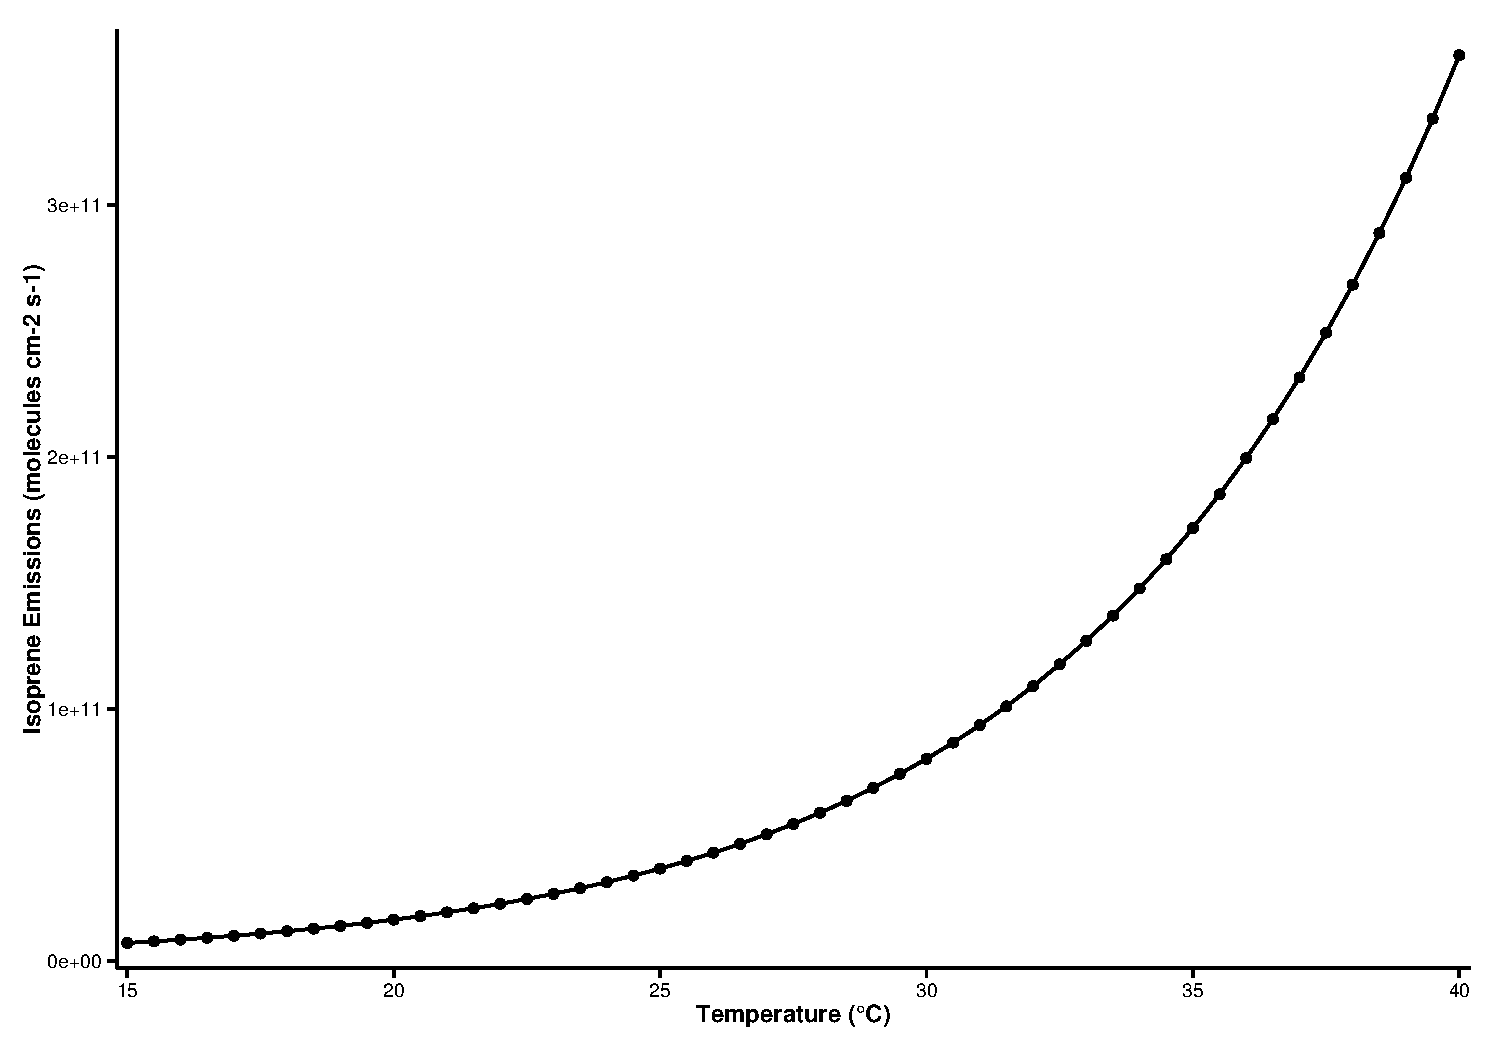
\includegraphics[scale = 0.8]{img/isoprene_emissions}
\end{figure}
Temperature-dependent emissions of isoprene were estimated using the MEGAN2.1 algorithm for calculating the emissions of VOC from vegetation \citep{Guenther:2012}.
Emissions from nature are dependent on many variables including temperature, radiation and age but for the purpose of our study all variables except temperature were held constant.

The MEGAN2.1 parameters were chosen to give similar isoprene mixing ratios at $20$~\degree C to the temperature-independent emissions of isoprene in order to compare the effects of increased isoprene emissions with temperature.
The estimated emissions of isoprene with MEGAN2.1 using these assumptions are illustrated in Fig.~\ref{f:isoprene_emissions} and show the expected exponential increase in isoprene emissions with temperature \citep{Guenther:2006}.

The estimated emissions of isoprene at $20$~\degree C lead to $0.07$~ppbv of isoprene in our simulations while at $30$~\degree C, the increased emissions of isoprene using MEGAN2.1 estimations lead to $0.35$~ppbv of isoprene in the model.
A measurement campaign over Essen, Germany \citep{Wagner:2014} measured $0.1$~ppbv of isoprene at temperature $20$~\degree C and $0.3$~ppbv of isoprene were measured at $30$~\degree C.
The similarity of the simulated and observed isoprene mixing ratios indicates that the MEGAN2.1 variables chosen for calculating the temperature-dependent emissions of isoprene were suitable for simulating urban conditions over central Europe.
